%
% 卒論レジュメフォーマット Ver.2.0 pLaTeX版
%
\documentclass[twocolumn]{jarticle} % 2段組のスタイルを用いている

\usepackage{wuse_resume}
\usepackage{url}
\newcommand{\RQone}{ソースコードを自動生成できるコメントに含めるべき情報の種類は何か}
\newcommand{\RQtwo}{ソースコードを自動生成できるコメントの情報量はどの程度か}
\usepackage[dvipdfmx]{graphicx} 

\newcommand{\todo}[1]{\colorbox{yellow}{{\bf TODO}:}{\color{red} {\textbf{[#1]}}}}
% \url{}コマンド用.URLを表示する際に便利
%\usepackage[dvipdfmx]{graphicx}  % ←graphicx.styを用いてEPSを取り込む場合有効にする
			% 他のパッケージ・スタイルを使う場合には適宜追加

%%%%%%%%%%%%%%%%%%%%%%%%%%%%%%%%%%%%%%%%%%%%%%%%%%%%%%%%%%%%%%%%%%%%%%%%

%%
%% タイトル,学生番号,氏名などを設定する
%%

\タイトル{コードレビューコメントの特徴によるソースコード自動修正の精度の比較}
\研究室{ソーシャルソフトウェア工学}
\学生番号{60266003}
\氏名{赤松 汰輝}

\概要{%
本研究では,レビューコメントの特徴がソースコード自動修正の精度に与える影響を分析する.コードレビューはソースコードの品質向上のために開発プロセスとして広く採用されているが,レビューアの指摘方法が適切でない,または情報量が不足していることにより実装者が正確に理解できないことがある.本研究では,GitHubから収集したレビューコメントに対して,修正の種類(リファクタリング,バグ,パフォーマンス)と指摘方法(エラー内容,再現方法,具体的な修正方法)の観点からラベル付けを行い,それぞれの条件における自動修正の精度を分析する.また,レビューコメントの情報量を変更した場合の精度も評価する.
}

\キーワード{コードレビュー}
\キーワード{コード自動修正}
\キーワード{GitHub}
\キーワード{機械学習}
\キーワード{Java}

%%%%%%%%%%%%%%%%%%%%%%%%%%%%%%%%%%%%%%%%%%%%%%%%%%%%%%%%%%%%%%%%%%%%%%%%

%% 以下の3行は変更しない

\begin{document}
\maketitle
\thispagestyle{empty} % タイトルを出力したページにもページ番号を付けない

%%%%%%%%%%%%%%%%%%%%%%%%%%%%%%%%%%%%%%%%%%%%%%%%%%%%%%%%%%%%%%%%%%%%%%%%

%%
%% 本文 - ここから
%%

\section{はじめに}

近年ソフトウェア開発はソフトウェアの大規模化や複雑化により,個人で行うのではなく,複数人で行うことが主流になっている.その中で,ソースコードレビュー(以後,コードレビュー)はソフトウェア開発において複数の開発者が協力して行う品質管理活動である.特に,検証作業を複数人のレビューアが取り組むことで,ソースコードの品質が向上する\cite{mcintosh2014impact}.

大規模なプロジェクトでは1ヶ月に数百件以上の検証依頼があり\cite{rigby2013convergent},これらを効率的に処理するためにはレビューアが指摘を正確かつ簡潔に実装者に伝え,コミュニケーションの回数を少なく抑えることが期待されるが,レビューアと実装者のコミュニケーションにおいて,レビューアの意図が正確に伝わらないケースがある.その結果,追加の確認や説明が必要になり,レビュー完了までの時間が長期化するという課題がある.

従来研究\cite{tufano2022using}では,コードレビューにかかるコスト軽減を目的とした自動修正モデルを提案しているが,レビューコメントの情報の種類や量が精度に与える影響については十分な分析がなされていない.そこで本研究では,以下の2つのResearch Question(RQ)を設定し,効果的なレビューコメントの特徴を理解することを目的とする.
\begin{itemize}
\item RQ1:\RQone
\item RQ2:\RQtwo
\end{itemize}

\if0
\section{事前分析}

\subsection{事前分析の目的}

従来研究では,コード生成タスクの評価指標として CodeBLEU スコアが使用されているが,入力されるソースコードの規模によってスコアが大きく変動することが観察されている.例えば,大規模なコードに対する小規模な修正では,修正の質に関わらず高いスコアが付与される傾向がある.したがって,レビューコメントの特徴がコード生成の精度に与える影響を正確に分析するためには,CodeBLEU スコアを評価指標として使用する際の適切なソースコード規模を明らかにする必要がある.そのため,本章では,コード自動修正モデルの評価指標であるCodeBLEUスコアを適切に使用するために,評価対象とすべきソースコードの規模を明らかにすることを目的とする.

\subsection{分析方法}

本分析では従来研究\cite{tufano2022using}で分析されていたGitHubおよびGerritリポジトリからコードレビュー関連のデータ167,799件を対象にする.分析に先立ち,データの前処理として2つの手順を実施した.まず,入力コードのノード数と変更ノード数について,四分位範囲(IQR)を用いて外れ値を除去した.次に,入力コードのノード数に基づいて,データを4つのグループ(Q1未満,Q1-Q2,Q2-Q3,Q3以上)に分割し,コードの規模による分析を可能とした.
変更箇所の特定においては,抽象構文木(AST)を用いた差分分析を実施した.具体的には,GumTreeツールを使用して,提出されたメソッドと修正後のメソッドの間で行われた変更を4種類の操作(追加,削除,更新,移動)として特定した.

\subsection{結果}

\fi

\section{RQ1:\RQone}

\subsection{分析方法}

本分析では従来研究\cite{tufano2022using}で分析されていたGitHubおよびGerritリポジトリからコードレビュー関連のデータ167,799件を対象にした.レビューコメントに含まれる情報の種類を分析するため,各レビューコメントに対して2つの観点からラベル付けを行った.
1つ目の観点はコンテキストである.レビューアが指摘している修正の背景や目的を分類するため,以下の3つのカテゴリを設定した:
\begin{itemize}
\item リファクタリング:コードの可読性や保守性を向上させるための修正
\item バグ:プログラムの不具合や意図しない動作の修正
\item パフォーマンス:実行速度やメモリ使用量などの性能に関する修正
\end{itemize}
2つ目の観点は修正依頼方法である.レビューアがどのような形で修正を依頼しているかを分類するため,以下の3つのカテゴリを設定した:
\begin{itemize}
\item エラーの内容の提示:発生している問題や不具合の内容を説明
\item 再現方法の提示:問題が発生する条件や手順を説明
\item 具体的な修正方法の提示:どのように修正すべきかの具体的な方法を説明
\end{itemize}

\subsection{結果}
レビューコメントの分析結果について,コンテキストの観点から得られたCodeBLEUスコアの分布に関しては,リファクタリング,バグ,パフォーマンスの3種類のコンテキスト間でCodeBLEUスコアの分布に大きな差は見られなかった.


\begin{figure}[htbp]
\centering
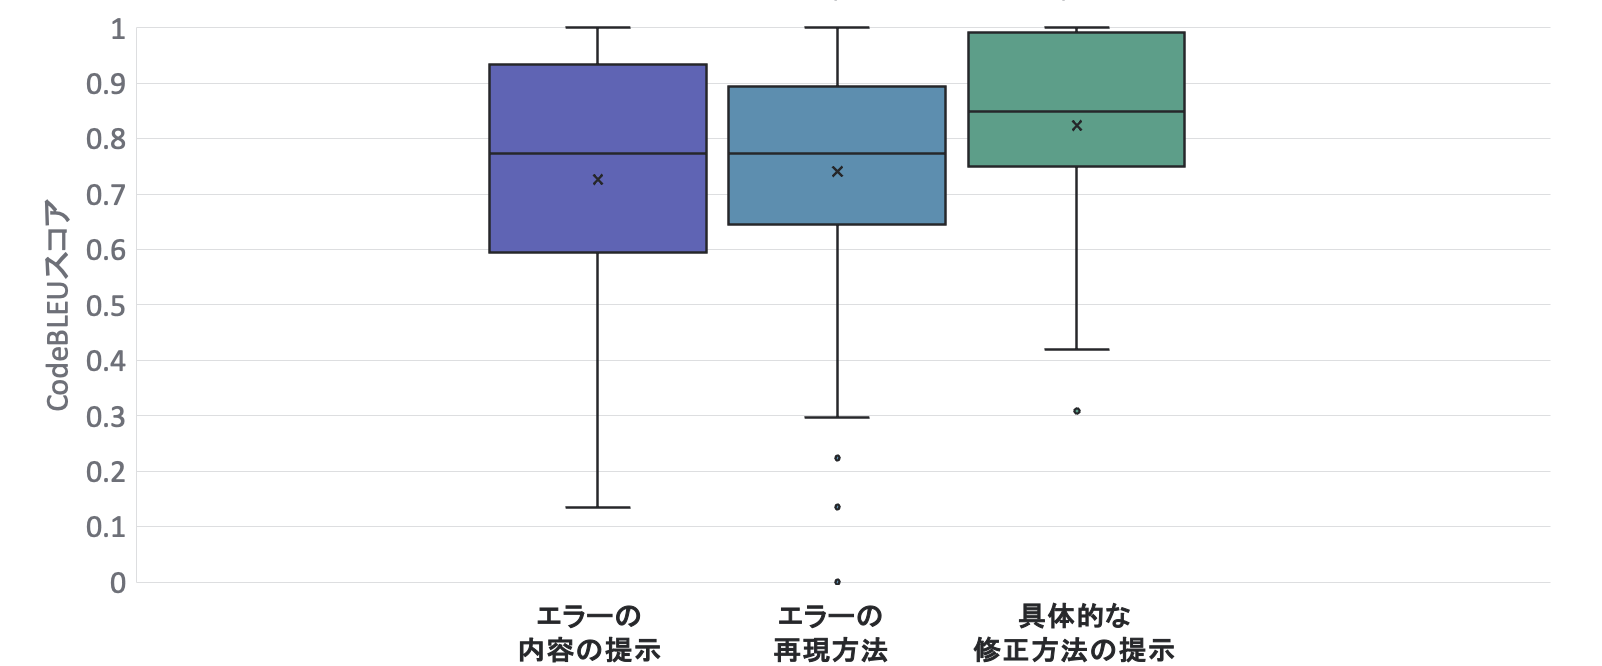
\includegraphics[width=0.8\linewidth]{@BSthesis2024_Akamatsu/Akamatsu_figs/rq1_result03_03.png}
\caption{修正依頼方法の違いによるCodeBLEUスコアの分布比較}
\label{fig:method-score}
\end{figure}

一方,修正依頼方法の観点からの分析結果を図\ref{fig:method-score}に示す.具体的な修正方法の提示が最も高いCodeBLEUスコアを示し(中央値:0.85,IQR:0.75-0.95),次いでエラーの再現方法(中央値:0.74,IQR:0.65-0.89),エラーの内容の提示(中央値:0.72,IQR:0.60-0.93)という順序となった.特筆すべき点として,具体的な修正方法を提示するコメントでは,スコアの分布が上位に集中し,より安定した高精度なコード生成を実現していた.


\section{RQ2:\RQtwo}

\subsection{分析方法}
本分析では,GitHubから収集したPull Request(PR)とそれに関連するデータを対象7,079件を対象とした.コード自動修正のアプローチとして,3つの手法を実施した.1つ目は基本的なレビューコメントとソースコードのみを用いた最小限の入力による手法(origin生成コード),2つ目はPull Requestから得られる追加情報を機械的に連結して入力とする手法(append生成コード),3つ目は基本レビューコメントとPull Request情報をGPT-4に入力し,より自然な形で文脈を補完した拡張レビューコメントを生成する手法である.なお,GPT-4の利用にあたってはgpt-4o-miniモデルを使用し,temperatureは0.7に設定した.これらを,コード自動修正モデルに入力し,コード生成の精度を比較した.

\subsection{結果}
1つ目は,GPTによるレビューコメント拡張の有効性である.GPTで拡張したexpand生成コードは,CodeBLEUスコアの中央値が約0.5(四分位範囲:0.3-0.8)となり,単純に情報を追加したappend生成コード(中央値約0.2,四分位範囲:0.1-0.3)と比較して有意に高いスコアを示した.これは,GPTがPull Requestの情報から有用な情報を選択的に抽出し,より具体的で文脈を考慮したレビューコメントを生成できることを示している.

2つ目は,レビューコメントの拡張パターンに関する分析結果である.

\begin{figure}[htbp]
\centering
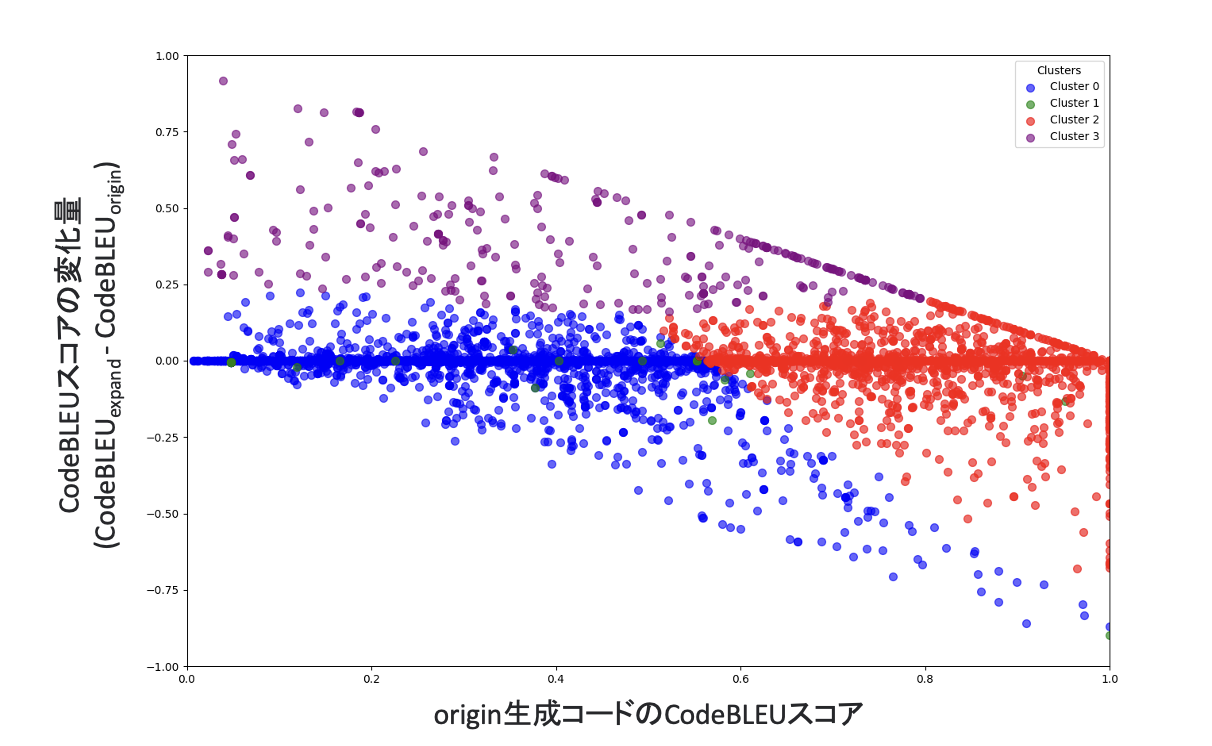
\includegraphics[width=0.9\linewidth]{@BSthesis2024_Akamatsu/Akamatsu_figs/rq2_result02_02.png}
\caption{元のCodeBLEUスコアとスコア変化量の関係}
\label{fig:scatter-cluster}
\end{figure}

図\ref{fig:scatter-cluster}は,横軸に元のCodeBLEUスコア,縦軸にスコアの変化量をとり,各データポイントをクラスタごとに色分けした散布図を示している.この図から,以下の4つの特徴的なクラスタの分布が確認できる.7,079件のレビューコメントを分析した結果,4つの特徴的なクラスタが確認され,特に改善成功グループでは,コードの具体的な部分を指摘し,約230文字程度の適度な長さで情報を提供することで,平均0.365のスコア向上を達成した.

\section{おわりに}

本研究では,コードレビューコメントの特徴が自動修正精度に与える影響を2つの観点から分析した.1つ目の分析では,レビューコメントの情報を「コンテキスト」と「修正依頼方法」の観点から調査し,修正の種類による精度の違いは限定的である一方,具体的な修正方法を示すコメントが高い精度を実現することを明らかにした.2つ目の分析では,GPTを用いたレビューコメントの拡張を検証し,200-250文字程度の適切な長さで,具体的な技術要素への言及を含む拡張が最も効果的であることを示した.これらはレビューコメントから自動的にコード修正を生成する際に,どのような情報が必要であり,どの程度の情報量が適切かを明らかにした.


%%
%% 本文 - ここまで
%%

%%%%%%%%%%%%%%%%%%%%%%%%%%%%%%%%%%%%%%%%%%%%%%%%%%%%%%%%%%%%%%%%%%%%%%%%

%%
%% 参考文献
%%

\bibliographystyle{junsrt}
\bibliography{@BSthesis2024_Akamatsu/BSthesis2024_Akamatsu}



%%%%%%%%%%%%%%%%%%%%%%%%%%%%%%%%%%%%%%%%%%%%%%%%%%%%%%%%%%%%%%%%%%%%%%%%

\end{document}
